\section{States} 

We present the two standard representations of quantum states used in quantum computing: the matrix (vector) representation and the Dirac notation.
%
We then introduce our tree-based representation.
%
We begin with the special case of classical states.

In classical computing, bits are the fundamental units of information. 
%
Each bit can exist in one of two possible states: 0 or 1. 
%
These may be conceptualized as switches that are either turned on or off. 
%
In contrast, quantum computing employs quantum bits, or {\it qubits}, to represent and process information. 
%
Qubits can exist in a {\it superposition}, meaning they may simultaneously be in state 0, state 1, or a combination of both. 
%
Additionally, a qubit can be subjected to a {\it measurement} operation. 
%
The state of a qubit is described by two complex numbers, called {\it amplitudes}, $c_0$ and $c_1$, where $|c_0|^2$ denotes the probability of measuring the state as $0$, and $|c_1|^2$ the probability of measuring it as $1$. 
%
These amplitudes must satisfy the normalization condition: $|c_0|^2 + |c_1|^2 = 1$.

\begin{figure}
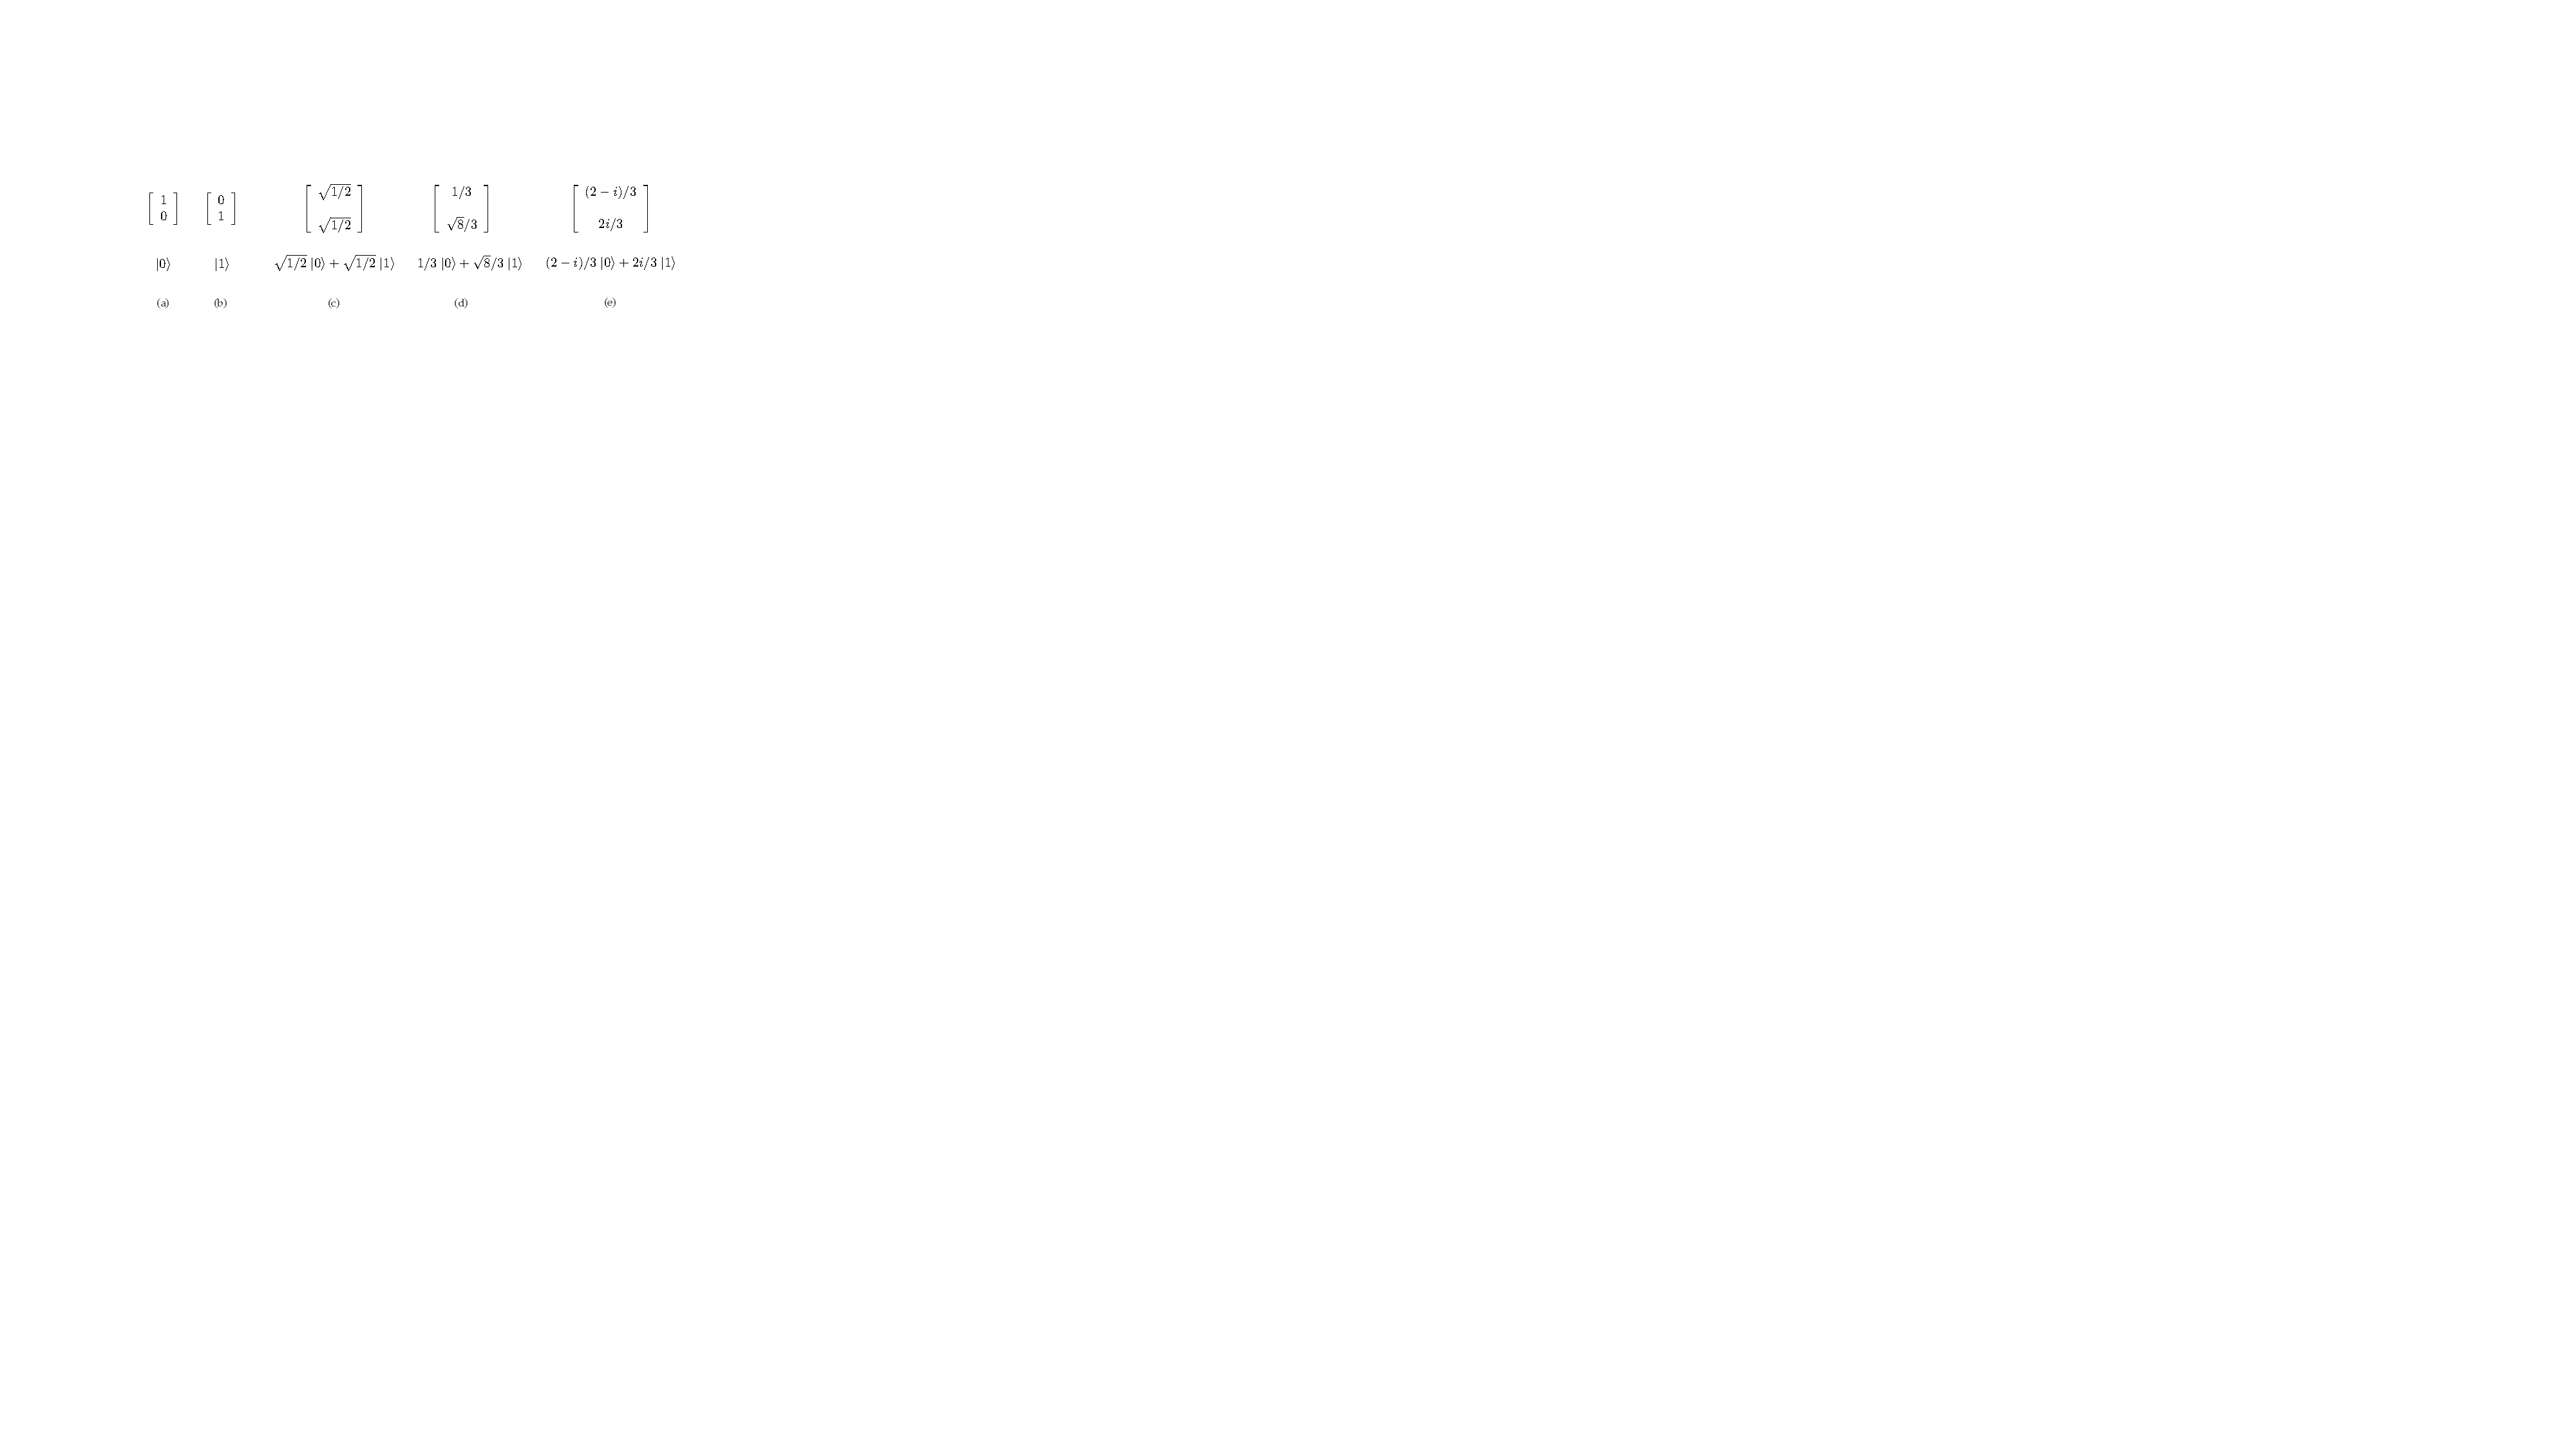
\includegraphics[scale=0.85]{Figures/States/states}
\caption{Different qubits and their vector and Dirac representations.
(a, b) The basis states $\ketof{0}$ and $\ketof{1}$.
(c, d, e) Quantum states in superposition.
%
Measuring the state in (c) yields $0$ or $1$ with probability $0.5$.
%
Measuring the state in (d) yields $0$ with probability $1/9$ and $1$ with probability $8/9$.
}
\label{qbit:state:fig}
\end{figure}

There are two common representations used to describe a qubit state (cf.\ \cref{qbit:state:fig}).
%
The first is the vector notation, in which the state is written as a column vector of length 2, with complex entries corresponding to the amplitudes of the respective basis states.
%
To simplify notation, we often use the transpose of this column vector.
%
For example, we write $[1/3\;\;\;\sqrt{8}/3]^T$ to represent the state shown in \cref{qbit:state:fig}~(d).
%
This results in a more compact row vector form.
%
The second representation is the Dirac notation, where the state is expressed as a linear combination, e.g., $\ketof{0} + \ketof{1}$.
%
Classical states are special cases where either $c_0 = 1$ and $c_1 = 0$, or $c_0 = 0$ and $c_1 = 1$.
%
In quantum systems, these are referred to as the basis states $\ketof{0}$ and $\ketof{1}$.

We now generalize these concepts to systems with multiple qubits.
%
For $n$ qubits, there are $2^n$ possible basis states.
%
%
In the case of two qubits, the system has four basis states.
%
These can be represented as column vectors:
\[
\left[
1\;0\;0\;0
\right]^{\mathtt T}
\;\;\;
\left[
0\;1\;0\;0
\right]^{\mathtt T}
\;\;\;
\left[
0\;0\;1\;0
\right]^{\mathtt T}
\;\;\;
\left[
0\;0\;0\;1
\right]^{\mathtt T}
\]

\begin{figure}
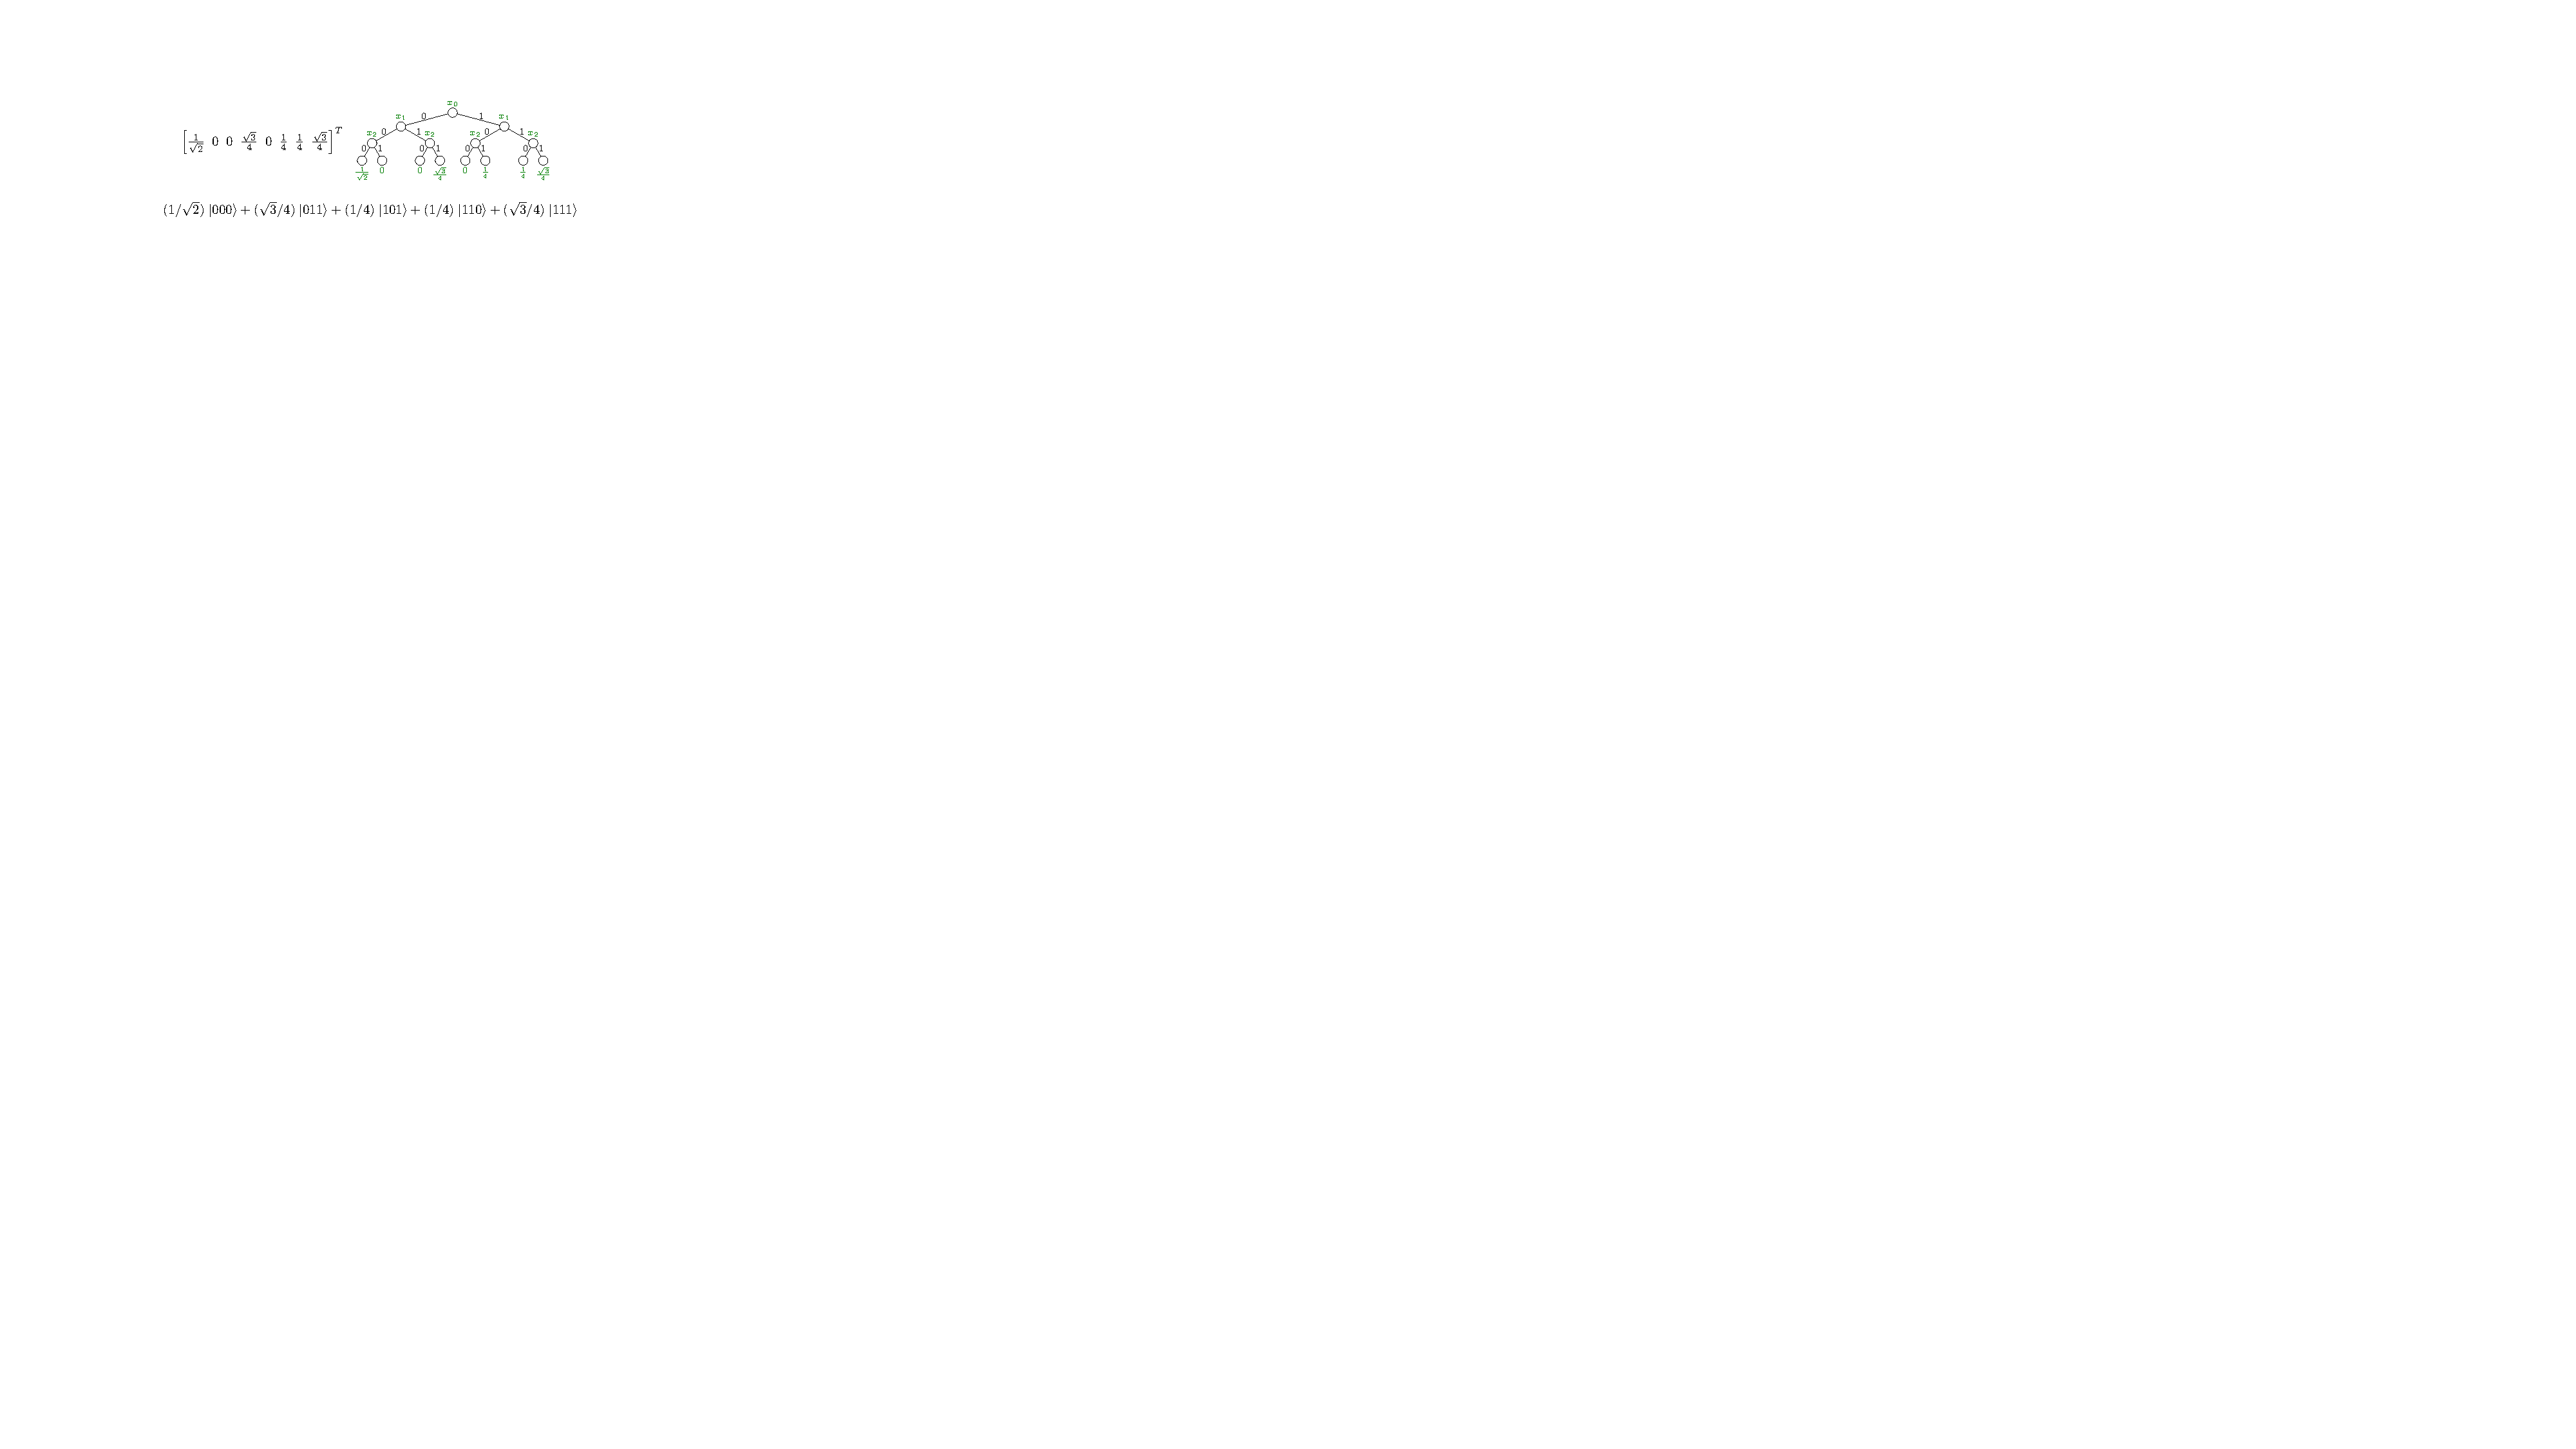
\includegraphics[scale=1]{Figures/States/state3}
\caption{A state involving three qubits.  We provide the vector, Dirac, and tree-based representations.
%
The tree spans all basis states, with the corresponding amplitudes shown as leaf labels.
%
For instance, the left-most path represents $\ketof{000}$ with amplitude $1/\sqrt{2}$.
}
\label{triple:qbit:state:fig}
\end{figure}


A key feature of our framework is a symbolic representation of quantum states and sets of quantum states.
%
We utilize {\it tree automata} as the underlying symbolic structure.
%
Specifically, a quantum state over $\nn$ qubits is encoded as a perfect binary tree of depth $\nn$.
%
Each level of the tree corresponds to one qubit.
%
We refer to the level associated with qubit $\xvar$ as the $\xvar$-level, and the nodes at that level as $\xvar$-nodes.
%
For any $\xvar$-node, its left and right subtrees represent the cases where qubit $\xvar$ has values $0$ and $1$, respectively.
%
Each root-to-leaf path encodes a computational basis state.
%
The leaf nodes hold the complex amplitudes associated with those basis states.

Consider \cref{triple:qbit:state:fig}.
%
The left side shows a quantum state involving three qubits.
%
The right side displays its corresponding tree representation.
%
